% ---- figures, generated -------------------------------------------
\newcommand{\NLetters}{52}
\newcommand{\NMeanings}{95}
\newcommand{\NCellsUsed}{59}
\newcommand{\NCellsTotal}{63}
\newcommand{\NShared}{23}
\newcommand{\NThreeWay}{9}
\newcommand{\NChecks}{12}
\newcommand{\NChecksPassed}{11}

\newcommand{\AlphabetTable}{%
% generated by make_paper_tables.py -- do not edit
\begin{LTR}
\begin{longtable}{llll llll}
\toprule
\sd{ا} & \bcell{1} & \sd{ب} & \bcell{1,2} & \sd{ٻ} & \bcell{2,6} & \sd{ڀ} & \bcell{2,3} \\
\sd{ت} & \bcell{2,3,4,5} & \sd{ٿ} & \bcell{1,2,5,6} & \sd{ٽ} & \bcell{2,4,6} & \sd{ٺ} & \bcell{1,3,5} \\
\sd{ث} & \bcell{1,4,5,6} & \sd{پ} & \bcell{1,2,3,4} & \sd{ج} & \bcell{2,4,5} & \sd{ڄ} & \bcell{3,5,6} \\
\sd{ڃ} & \bcell{3,5} & \sd{چ} & \bcell{1,4} & \sd{ڇ} & \bcell{1,6} & \sd{ح} & \bcell{1,5,6} \\
\sd{خ} & \bcell{1,3,4,6} & \sd{د} & \bcell{1,4,5} & \sd{ڌ} & \bcell{1,2,3,6} & \sd{ڏ} & \bcell{3,4} \\
\sd{ڊ} & \bcell{3,4,6} & \sd{ڍ} & \bcell{2,5,6} & \sd{ذ} & \bcell{2,3,4,6} & \sd{ر} & \bcell{1,2,3,5} \\
\sd{ڙ} & \bcell{1,2,4,5,6} & \sd{ز} & \bcell{1,3,5,6} & \sd{س} & \bcell{2,3,4} & \sd{ش} & \bcell{1,4,6} \\
\sd{ص} & \bcell{1,2,3,4,6} & \sd{ض} & \bcell{1,2,4,6} & \sd{ط} & \bcell{2,3,4,5,6} & \sd{ظ} & \bcell{1,2,3,4,5,6} \\
\sd{ع} & \bcell{1,2,3,5,6} & \sd{غ} & \bcell{1,2,6} & \sd{ف} & \bcell{1,2,4} & \sd{ڦ} & \bcell{2,3,5} \\
\sd{ق} & \bcell{1,2,3,4,5} & \sd{ڪ} & \bcell{1,3} & \sd{ک} & \bcell{1,3} \bcell{2,3,6} & \sd{گ} & \bcell{1,2,4,5} \\
\sd{ڳ} & \bcell{1,3,4,5,6} & \sd{ڱ} & \bcell{2,3,5,6} & \sd{ل} & \bcell{1,2,3} & \sd{م} & \bcell{1,3,4} \\
\sd{ن} & \bcell{1,3,4,5} & \sd{ڻ} & \bcell{3,4,5,6} & \sd{و} & \bcell{2,4,5,6} & \sd{ه} & \bcell{1,2,5} \\
\sd{ھ} & \bcell{2,3,6} & \sd{ي} & \bcell{2,4} & \sd{ء} & \bcell{3} & \sd{آ} & \bcell{3,4,5} \\
\bottomrule
\end{longtable}
\end{LTR}
}

\newcommand{\AmbiguityTable}{%
% generated by make_paper_tables.py -- do not edit
\begin{LTR}\footnotesize
\begin{longtable}{clp{0.31\linewidth}p{0.34\linewidth}}
\caption{Every cell the code assigns more than one reading, with the criterion that resolves it. Generated from the implemented tables.}\label{tab:ambiguity}\\
\toprule
cell & dots & readings & resolved by \\
\midrule\endhead
\bcell{2} & \texttt{2} & zabar (diacritic); comma (punctuation); 1 (lower digit); decimal point (sign); pen-name mark (sign) & diacritic after a letter · comma after a completed word · decimal point inside a number · lower 1 after a number sign · and immediately before a pen-name in verse \\[2pt]
\bcell{2,5} & \texttt{25} & jazam (diacritic); colon (punctuation); 3 (lower digit); ratio mark (sign) & colon or jazam in prose · ratio when a fresh number sign follows · lower 3 after a number sign \\[2pt]
\bcell{3,5} & \texttt{35} & \sd{ڃ} (letter); double zer (diacritic); 9 (lower digit); footnote mark (sign) & letter · diacritic after a letter · lower digit after a number sign · the same cell twice is a footnote \\[2pt]
\bcell{3} & \texttt{3} & \sd{ء} (letter); doubling mark (sign); blank line (sign) & the letter \sd{ء} inside a word · the same cell twice after a word means the word is repeated · three of them is a blank line \\[2pt]
\bcell{2,3} & \texttt{23} & \sd{ڀ} (letter); semicolon (punctuation); 2 (lower digit) & letter inside a word · semicolon at the end · lower digit after a number sign \\[2pt]
\bcell{2,6} & \texttt{26} & \sd{ٻ} (letter); double pesh (diacritic); 5 (lower digit) & letter · diacritic after a letter · lower digit after a number sign \\[2pt]
\bcell{2,3,5} & \texttt{235} & \sd{ڦ} (letter); exclamation (punctuation); 6 (lower digit) & letter inside a word · exclamation at the end · lower digit after a number sign \\[2pt]
\bcell{2,3,6} & \texttt{236} & \sd{ھ} (letter); question (punctuation); 8 (lower digit) & never fully resolves. The letter \sd{ھ} by default at the end of a word; a word list recovers \sd{؟} \\[2pt]
\bcell{2,5,6} & \texttt{256} & \sd{ڍ} (letter); full stop (punctuation); 4 (lower digit) & letter inside a word · full stop at the end · lower digit after a number sign \\[2pt]
\bcell{1} & \texttt{1} & \sd{ا} (letter); 1 (digit) & letter inside a word; the other reading only in its own position \\[2pt]
\bcell{1,2} & \texttt{12} & \sd{ب} (letter); 2 (digit) & letter inside a word; the other reading only in its own position \\[2pt]
\bcell{1,4} & \texttt{14} & \sd{چ} (letter); 3 (digit) & letter inside a word; the other reading only in its own position \\[2pt]
\bcell{1,5} & \texttt{15} & zer (diacritic); 5 (digit) & zer after a letter; the digit only after a number sign \\[2pt]
\bcell{2,4} & \texttt{24} & \sd{ي} (letter); 9 (digit) & letter inside a word; the other reading only in its own position \\[2pt]
\bcell{1,2,4} & \texttt{124} & \sd{ف} (letter); 6 (digit) & letter inside a word; the other reading only in its own position \\[2pt]
\bcell{1,2,5} & \texttt{125} & \sd{ه} (letter); 8 (digit) & letter inside a word; the other reading only in its own position \\[2pt]
\bcell{1,4,5} & \texttt{145} & \sd{د} (letter); 4 (digit) & letter inside a word; the other reading only in its own position \\[2pt]
\bcell{2,4,5} & \texttt{245} & \sd{ج} (letter); 0 (digit) & letter inside a word; the other reading only in its own position \\[2pt]
\bcell{3,5,6} & \texttt{356} & \sd{ڄ} (letter); 0 (lower digit) & letter inside a word; the other reading only in its own position \\[2pt]
\bcell{1,2,4,5} & \texttt{1245} & \sd{گ} (letter); 7 (digit) & letter inside a word; the other reading only in its own position \\[2pt]
\bcell{2,3,5,6} & \texttt{2356} & \sd{ڱ} (letter); 7 (lower digit) & letter inside a word; the other reading only in its own position \\[2pt]
\bcell{3,4,5,6} & \texttt{3456} & \sd{ڻ} (letter); number sign (sign) & number sign at the start of a word, \sd{ڻ} everywhere else. No ordinary word begins with \sd{ڻ}. The aspirate \sd{ڻھ} does, and its two cells are also the fraction 1/8, which is why it is one of the four spellings this code cannot read back \\[2pt]
\bcell{1,2,3,5,6} & \texttt{12356} & \sd{ع} (letter); verse mark (sign) & \sd{ع} inside a word · twice at the head of a stanza, and once at the end of each line, is verse \\[2pt]
\bottomrule
\end{longtable}
\end{LTR}
}

\newcommand{\VerificationTable}{%
% generated by make_paper_tables.py -- do not edit
\begin{LTR}\small
\begin{tabular}{llp{0.60\linewidth}}
\toprule
 & check & what it reports \\
\midrule
\pass & \texttt{guide} & 68 of 68 printed examples, cell for cell and space for space; 1 known divergence, see verify\_guide.DIVERGENCE \\
\pass & \texttt{rules} & 10 of 10 stated rules — implemented as read, not evidence \\
\pass & \texttt{selftest} & 14 exact   2 equivalent spelling   0 wrong   (16/16 faithful) \\
\pass & \texttt{words} & 99.94\% of 23432 words survive the round trip (4 spellings do not: \sd{عيسوي،} \sd{تعالي،} \sd{صلعم،} \sd{ڻھ}) \\
\pass & \texttt{grade2} & 238 of 243 contractions round trip; the 5 that do not are cells the book itself gives to two words \\
\pass & \texttt{sheets} & the print sheets and the check sheet rebuild unchanged \\
\pass & \texttt{neighbours} & 94 of 99 shared letters agree with Arabic, Persian and Urdu; the 5 that differ are letters those codes do not have \\
\pass & \texttt{ambiguity} & the site lists all 23 cells that carry more than one reading \\
\pass & \texttt{wordlist} & the browser is carrying the same 2702 words \\
\skipped & \texttt{liblouis} & liblouis tools not installed — not checked \\
\pass & \texttt{browser} & 70 of 70 cases agree between the browser and the Python \\
\pass & \texttt{document} & a 36-page document converts identically in the browser and here \\
\bottomrule
\end{tabular}
\end{LTR}
}

\newcommand{\ReadingsHistogram}{%
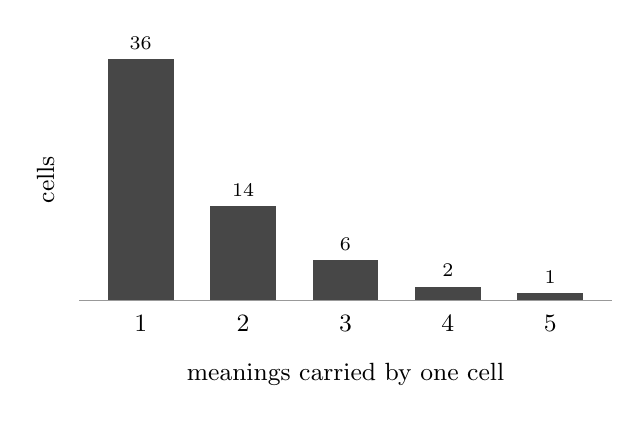
\begin{tikzpicture}[x=13mm, y=9mm]
\draw[black!40] (0.4,0) -- (5.6,0);
\draw[fill=black!72, draw=none] (1-0.32,0) rectangle (1+0.32,3.400);
\node[font=\scriptsize, anchor=south] at (1,3.400) {36};
\draw[fill=black!72, draw=none] (2-0.32,0) rectangle (2+0.32,1.322);
\node[font=\scriptsize, anchor=south] at (2,1.322) {14};
\draw[fill=black!72, draw=none] (3-0.32,0) rectangle (3+0.32,0.567);
\node[font=\scriptsize, anchor=south] at (3,0.567) {6};
\draw[fill=black!72, draw=none] (4-0.32,0) rectangle (4+0.32,0.189);
\node[font=\scriptsize, anchor=south] at (4,0.189) {2};
\draw[fill=black!72, draw=none] (5-0.32,0) rectangle (5+0.32,0.094);
\node[font=\scriptsize, anchor=south] at (5,0.094) {1};
\foreach \k in {1,...,5}{\node[font=\small, anchor=north] at (\k,-0.08) {\k};}
\node[font=\small, anchor=north] at (3.0,-0.75) {meanings carried by one cell};
\node[font=\small, rotate=90, anchor=south] at (0.25,1.7) {cells};
\end{tikzpicture}}

\newcommand{\WorkedSindhi}{\sd{هن} \sd{۾} 8 + 9 = 17 \sd{آهي؟}}
\newcommand{\WorkedBack}{\sd{هن} \sd{۾} 8 + 9 =17 \sd{آهي؟}}
\newcommand{\WorkedGroups}{%
\begin{tabular}{ccccccc}
\bcell{1,2,5} \bcell{1,3,4,5} & \bcell{1,3,4} \bcell{2,4} \bcell{1,3,4,5} & \bcell{3,4,5,6} \bcell{1,2,5} & \bcell{5,6} \bcell{2,3,5} & \bcell{3,4,5,6} \bcell{2,4} & \bcell{5,6} \bcell{2,3,5,6} \bcell{3,4,5,6} \bcell{1} \bcell{1,2,4,5} & \bcell{3,4,5} \bcell{1,2,5} \bcell{2,4} \bcell{2,3,6} \\[3pt]
{\scriptsize\ttfamily 125\,1345} & {\scriptsize\ttfamily 134\,24\,1345} & {\scriptsize\ttfamily 3456\,125} & {\scriptsize\ttfamily 56\,235} & {\scriptsize\ttfamily 3456\,24} & {\scriptsize\ttfamily 56\,2356\,3456\,1\,1245} & {\scriptsize\ttfamily 345\,125\,24\,236} \\
\end{tabular}}
\newcommand{\NWorkedGroups}{7}
